\documentclass[sigconf,screen,review,anonymous]{acmart}

\setcopyright{none}
\settopmatter{printacmref=false, printccs=false, printfolios=true}
\renewcommand\footnotetextcopyrightpermission[1]{}
\pagestyle{plain}

\usepackage{booktabs}
\usepackage{graphicx}
\usepackage{array}
\usepackage{float}
\usepackage{xcolor}
\usepackage{enumitem}
\usepackage{balance}

\setlist[itemize]{leftmargin=1.2em}
\setlist[enumerate]{leftmargin=1.4em}
\renewcommand{\arraystretch}{1.08}

\title{Weekly Report: Remote Data Sharing and Memory-Hierarchy Bottlenecks on Wafer-Scale GPUs}
\subtitle{Week ending June 1, 2026}

\begin{document}

\begin{abstract}
This report summarizes one week of work on understanding data sharing and remote
memory behavior on wafer-scale GPUs.  The main outcome is a shift from a broad
``data-sharing-aware scheduling'' idea to a more precise remote-access taxonomy.
Across traditional and ML workloads, high remote-access ratio is not by itself
evidence of a useful data-sharing optimization.  Remote traffic can come from
private placement mismatch, output/write ownership mismatch, shared read-mostly
reuse, or topology-local neighbor reuse.  New traces were added to classify
these cases at page granularity and to attribute remote reads to remote L2/MSHR
or remote DRAM service.
\end{abstract}

\ccsdesc[500]{Computer systems organization~Architectures}
\ccsdesc[300]{Computer systems organization~Heterogeneous systems}
\keywords{wafer-scale GPU, remote memory, data sharing, L2 cache, bottleneck analysis}

\maketitle

\section{Summary}

This week's work focused on turning page-sharing traces into architectural
evidence.  The main question was whether remote data access is a true
bottleneck, and if so, whether the right mechanism is page placement,
home-L2 caching, or a neighbor-exposed L2 hierarchy.

The strongest result is that remote accesses are heterogeneous.  For example,
SpMV has high remote traffic, high remote-DRAM service, high neighbor locality,
and a strong all-local oracle speedup.  This makes it the best current case for
remote data being on the critical path.  PageRank is different: its remote
traffic is more shared-read-mostly and mostly served by remote L2/MSHR, making
it a cleaner home-L2 candidate.  MatMul and AES are important negative controls:
they have high remote and sharing ratios, but the prior all-local oracle did
not improve performance.

\section{Complete Work Log}

\subsection{Research Framing}

The initial idea was to exploit cross-tenant data sharing in RAG-style
multi-tenant serving by grouping thread blocks around shared read-mostly data.
After looking at the available traces, the direction changed.  The current
benchmarks do not yet expose a clean tenant/request boundary, and the observed
data reuse is easier to reason about at page and GPU level than at thread-block
level.  The working framing is now:

\begin{quote}
Remote accesses on wafer-scale GPUs should first be classified.  Only a subset
of remote traffic is true shared read-mostly reuse; other traffic is placement
or output ownership mismatch.
\end{quote}

Related work was also re-positioned.  STAR is useful as a multi-tenant
benchmark-construction reference, but its main axis is destructive interference
in partitioned GPU environments.  This project instead targets constructive
reuse and topology-local remote data movement.  LADM is closer because it
studies locality-centric data and threadblock management for massive GPUs, but
the current traces do not yet provide an obvious thread-block level hook.  This
motivated the page-level and GPU-level trace work below.

\subsection{Experiment and Visualization Work}

The following analysis and visualization work was completed this week.

\begin{itemize}
  \item Generated chord diagrams and row-style requester-owner diagrams for
  remote access flows, including versions that cover 80\% of remote requests.
  \item Updated traditional wafer-flow maps so that all traditional workloads
  are plotted instead of a hand-selected subset.
  \item Added remote-access ratio annotations to the row-style diagrams.
  \item Added remote-page local-use analysis: whether a page remotely accessed
  by GPU A is also locally used by its owner GPU.
  \item Built an all-local data-access bottleneck copy of the codebase while
  keeping remote address translation through IOMMU.  This is used as an oracle
  to ask whether remote data movement is on the performance path.
  \item Compared bottleneck-analysis results against the original result
  directory only after checking problem signatures.
  \item Added bar plots for speedup-over-baseline and remote-access ratio.
  \item Added the new L2-source page-service trace and generated the latest
  traditional result set with it.
\end{itemize}

\subsection{Result Artifacts}

\begin{table*}[t]
  \centering
  \caption{Main result directories and report artifacts produced or used this week.}
  \label{tab:artifacts}
  \resizebox{\textwidth}{!}{\begin{tabular}{ll}
\toprule
Artifact & Path \\
\midrule
Traditional sharing traces & \texttt{akkalat/results/2026-05-26-01-59-52-translation-sweep} \\
Traditional L2-source run & \texttt{akkalat/results/2026-06-01-00-17-43-sampled-validation} \\
LLM sampled validation & \texttt{akkalat/results/2026-05-29-03-05-55-sampled-validation} \\
Traditional all-local oracle & \texttt{bottleneck analysis/akkalat/results/2026-05-29-18-10-44-traditional-bottleneck-analysis} \\
LLM all-local oracle & \texttt{bottleneck analysis/akkalat/results/2026-05-31-04-22-59-traditional-bottleneck-analysis} \\
Standalone report & \texttt{akkalat/results/weekly\_report\_2026-06-01} \\
ACM-template report & \texttt{weeklyreport/06012026} \\
\bottomrule
\end{tabular}
}
\end{table*}

\section{Instrumentation Completed}

\subsection{Page-Level Sharing Trace}

The page-sharing trace now records both virtual and physical page information:
\texttt{pid}, \texttt{page\_id}, \texttt{page\_vaddr},
\texttt{page\_paddr}, \texttt{page\_block}, \texttt{page\_size},
\texttt{paddr}, \texttt{bytes}, and \texttt{is\_write}.  Each run now emits a
per-page file, \texttt{*\_sharing\_pages.csv}, which summarizes read/write
ratio, local and remote accesses, sharer count, remote sharer count, dominant
owner, dominant requester, requester counts, owner counts, and reuse window.

\subsection{L2 Service-Source Trace}

The L2-source tracer now emits a compact page-level service file:
\texttt{*\_l2\_source\_page\_source.csv}.  The main fields are:
\texttt{source}, \texttt{requester\_gpm}, \texttt{provider\_gpm},
\texttt{hops}, \texttt{is\_neighbor}, \texttt{access\_type},
\texttt{page\_paddr}, \texttt{accesses}, \texttt{bytes},
\texttt{avg\_latency\_ns}, \texttt{first\_time\_ns}, and
\texttt{last\_time\_ns}.  This makes it possible to classify remote reads as
remote L2 cache hits, remote MSHR service, remote DRAM service, or 1-hop
neighbor service.

\subsection{Analysis Scripts}

The new post-processing script \texttt{analyze\_l2\_home\_evidence.py} joins
page-sharing summaries with L2-source traces and emits:
\texttt{l2\_home\_evidence\_pages.csv} and
\texttt{l2\_home\_evidence\_summary.csv}.  The key output metrics are
remote-read L2 service ratio, remote-read DRAM service ratio, neighbor-read
ratio, and a page-level classification into shared-read-mostly, owner-and-remote
use, remote-private mismatch, write/output mismatch, and local-only pages.

\section{Traditional Workload Results}

\begin{table}[t]
  \centering
  \caption{Selected traditional workloads. Remote L2 includes remote L2 cache
  hits and remote MSHR service. Neighbor means 1-hop requester-provider traffic.
  Shared-read and private are fractions of remote accesses after page-level
  classification.}
  \label{tab:traditional-selected}
  \resizebox{\columnwidth}{!}{\begin{tabular}{lrrrrrr}
\toprule
Benchmark & Remote & Remote L2 & Remote DRAM & Neighbor & Shared-read & Private \\
\midrule
spmv & 66.3 & 18.9 & 81.1 & 65.5 & 6.8 & 64.4 \\
pagerank & 31.8 & 91.8 & 8.2 & 18.3 & 70.9 & 29.1 \\
fastwalshtransform & 70.5 & 96.1 & 3.9 & 60.1 & 0.0 & 52.8 \\
fir & 69.5 & 91.1 & 8.9 & 70.7 & 1.5 & 93.7 \\
matrixmultiplication & 89.0 & 100.0 & 0.0 & 5.2 & 97.6 & 0.0 \\
aes & 94.8 & 6.3 & 93.7 & 80.0 & 99.8 & 0.2 \\
kmeans & 71.7 & 93.6 & 6.4 & 16.7 & 0.0 & 95.2 \\
stencil2d & 97.4 & 34.6 & 65.4 & 7.4 & 63.5 & 0.0 \\
nw & 97.9 & 25.1 & 74.9 & 5.7 & 12.3 & 34.3 \\
\bottomrule
\end{tabular}
}
\end{table}

Table~\ref{tab:traditional-selected} and
Figures~\ref{fig:traditional-taxonomy}--\ref{fig:traditional-scatter} summarize
the newest traditional run.  The result directory is
\texttt{akkalat/results/2026-06-01-00-17-43-sampled-validation}.

\begin{figure*}[t]
  \centering
  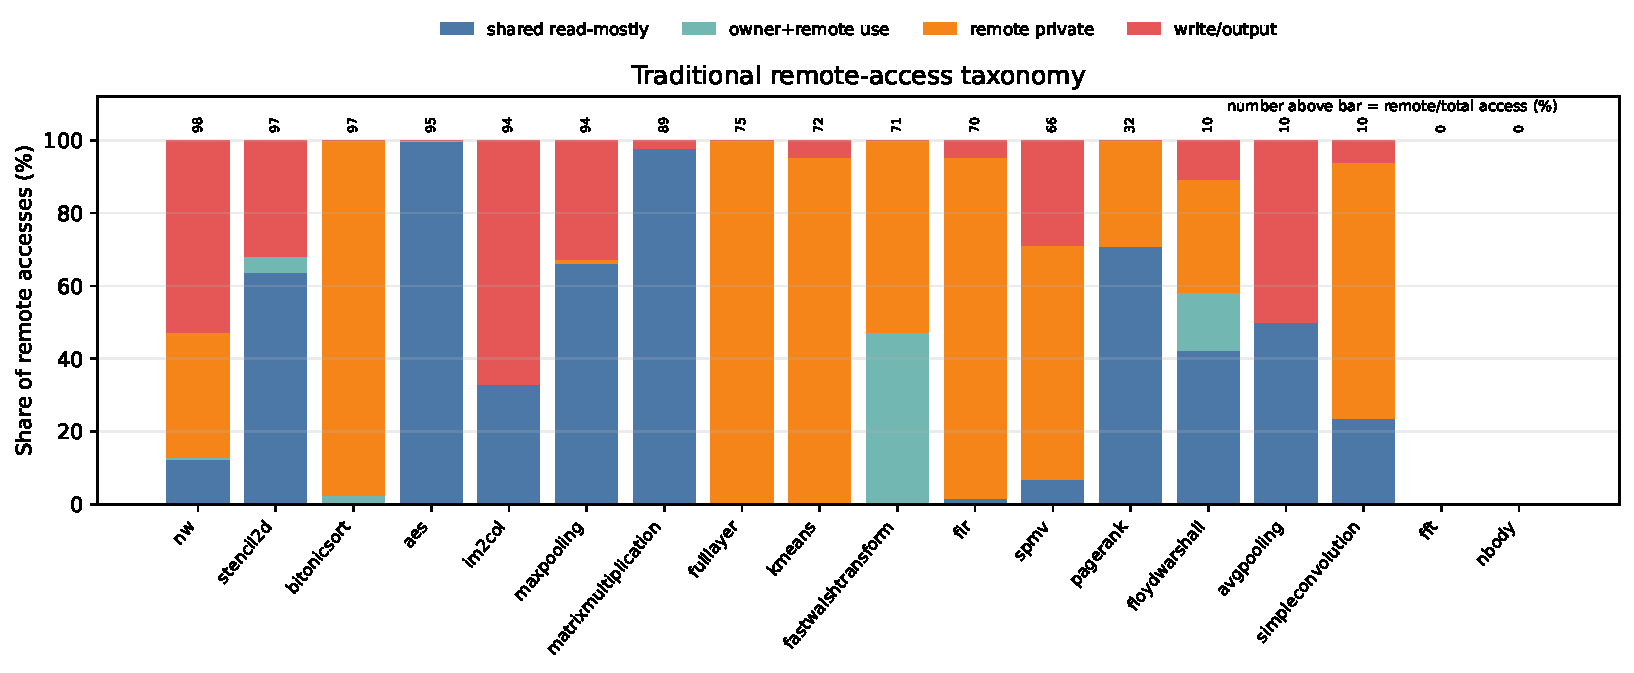
\includegraphics[width=0.98\textwidth]{figures/traditional_remote_taxonomy.pdf}
  \caption{Remote-access taxonomy for traditional workloads.  The number above
  each bar is the total remote-access ratio.  High remote ratio can mean very
  different things: shared read reuse, private placement mismatch, output/write
  mismatch, or a mixture.}
  \label{fig:traditional-taxonomy}
\end{figure*}

\begin{figure*}[t]
  \centering
  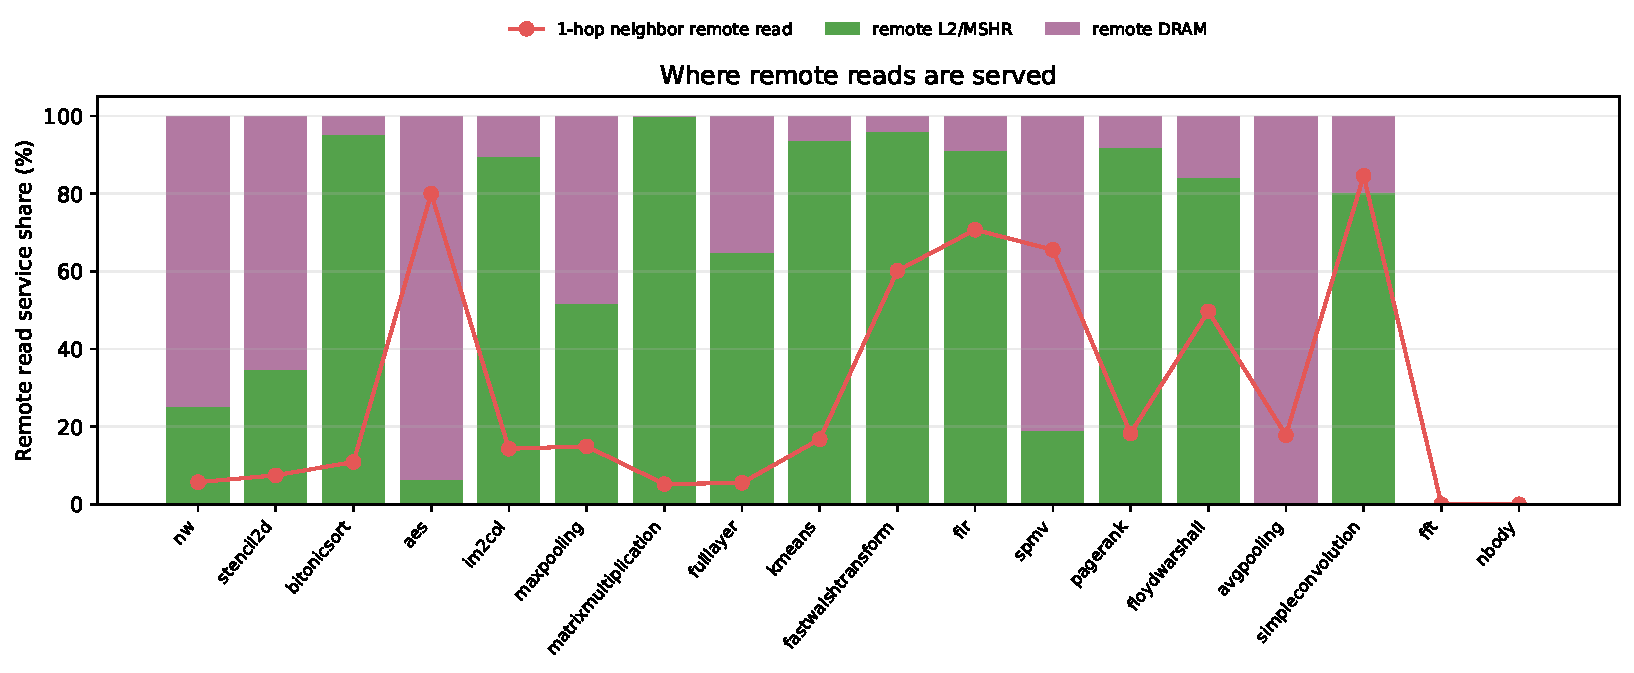
\includegraphics[width=0.98\textwidth]{figures/traditional_l2_service_neighbor.pdf}
  \caption{Remote read service source.  Some workloads are mostly served by
  remote L2/MSHR, while others still send a large fraction of remote reads to
  remote DRAM.  The red line shows the share of remote reads that are 1-hop
  neighbor accesses.}
  \label{fig:traditional-service}
\end{figure*}

\begin{figure}[t]
  \centering
  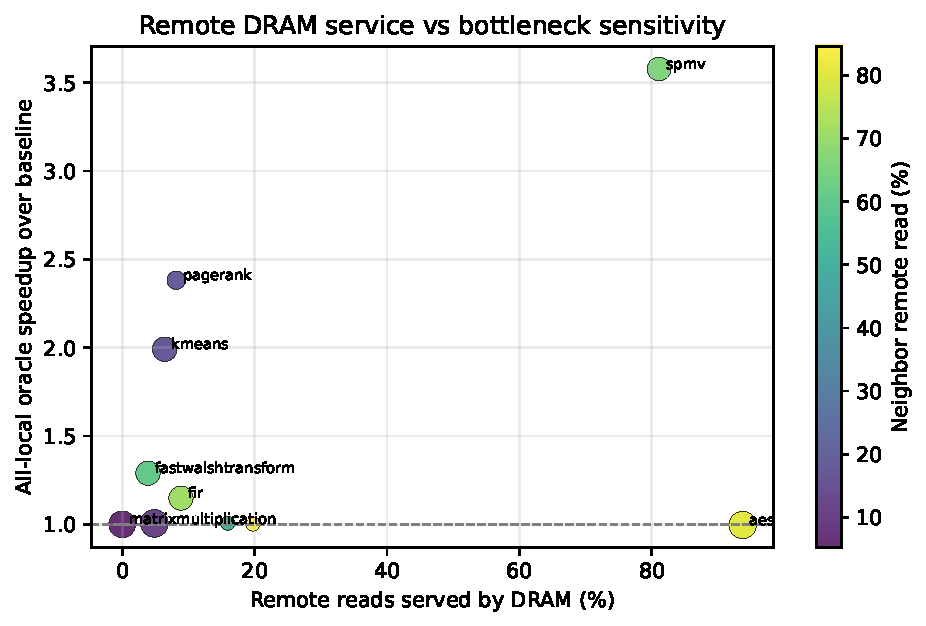
\includegraphics[width=\columnwidth]{figures/traditional_bottleneck_scatter.pdf}
  \caption{Remote DRAM service compared with prior all-local oracle speedup.
  SpMV is the strongest remote-data bottleneck.  PageRank also benefits, but its
  remote reads are mostly served by remote L2/MSHR, suggesting a different
  mechanism.}
  \label{fig:traditional-scatter}
\end{figure}

\subsection{Key Traditional Cases}

\textbf{SpMV} is the strongest bottleneck candidate.  It has 66.3\% remote
accesses, 81.1\% remote reads served by remote DRAM, 65.5\% neighbor remote
reads, and a prior all-local oracle speedup of 3.58$\times$.  This suggests
that remote data movement is on the critical path, but the traffic is not purely
shared read-mostly; much of it looks like placement or output mismatch.

\textbf{PageRank} is the cleanest shared-read/home-L2 candidate.  It has 31.8\%
remote accesses, 70.9\% shared-read-mostly remote traffic, 91.8\% remote
L2/MSHR service, and a prior all-local oracle speedup of 2.38$\times$.

\textbf{FWT} and \textbf{FIR} are good neighbor-L2 candidates.  They have high
remote ratios, most remote reads are served by remote L2/MSHR, and neighbor
remote reads are 60.1\% and 70.7\%, respectively.  These results motivate an L2
design that isolates local bandwidth from neighbor-facing bandwidth.

\textbf{MatMul} and \textbf{AES} are useful negative controls.  MatMul has
89.0\% remote accesses and 97.6\% shared-read-mostly remote traffic, but remote
reads are almost entirely served by L2/MSHR and prior all-local speedup is about
1.0$\times$.  AES also has high remote and shared-read ratios, but prior
all-local speedup is about 1.0$\times$.  These cases show that high remote ratio
and high sharing do not automatically imply performance opportunity.

\subsection{All Traditional Results}

Table~\ref{tab:traditional-all} reports the full traditional L2-source
classification result.  The columns are: total remote-access ratio; remote-read
service from L2/MSHR; remote-read service from DRAM; 1-hop neighbor remote-read
ratio; and four page-level classes as fractions of remote accesses.

\begin{table*}[t]
  \centering
  \caption{Full traditional workload remote-access taxonomy from the latest
  L2-source run.}
  \label{tab:traditional-all}
  \resizebox{\textwidth}{!}{\begin{tabular}{lrrrrrrrr}
\toprule
Benchmark & Remote & L2 & DRAM & Neighbor & Shared & Owner+R & Private & Write \\
\midrule
nw & 97.9 & 25.1 & 74.9 & 5.7 & 12.3 & 0.6 & 34.3 & 52.9 \\
stencil2d & 97.4 & 34.6 & 65.4 & 7.4 & 63.5 & 4.6 & 0.0 & 31.9 \\
bitonicsort & 97.2 & 95.2 & 4.8 & 10.9 & 0.0 & 2.4 & 97.6 & 0.0 \\
aes & 94.8 & 6.3 & 93.7 & 80.0 & 99.8 & 0.0 & 0.2 & 0.0 \\
im2col & 94.3 & 89.6 & 10.4 & 14.3 & 33.0 & 0.0 & 0.0 & 67.0 \\
maxpooling & 94.2 & 51.6 & 48.4 & 14.9 & 66.2 & 0.0 & 1.0 & 32.9 \\
matrixmultiplication & 89.0 & 100.0 & 0.0 & 5.2 & 97.6 & 0.0 & 0.0 & 2.4 \\
fulllayer & 75.2 & 64.8 & 35.2 & 5.5 & 0.0 & 0.0 & 100.0 & 0.0 \\
kmeans & 71.7 & 93.6 & 6.4 & 16.7 & 0.0 & 0.0 & 95.2 & 4.8 \\
fastwalshtransform & 70.5 & 96.1 & 3.9 & 60.1 & 0.0 & 47.2 & 52.8 & 0.0 \\
fir & 69.5 & 91.1 & 8.9 & 70.7 & 1.5 & 0.0 & 93.7 & 4.8 \\
spmv & 66.3 & 18.9 & 81.1 & 65.5 & 6.8 & 0.0 & 64.4 & 28.8 \\
pagerank & 31.8 & 91.8 & 8.2 & 18.3 & 70.9 & 0.0 & 29.1 & 0.0 \\
floydwarshall & 10.3 & 84.0 & 16.0 & 49.7 & 42.2 & 15.9 & 31.2 & 10.7 \\
avgpooling & 10.2 & 0.0 & 100.0 & 17.8 & 50.0 & 0.0 & 0.0 & 50.0 \\
simpleconvolution & 9.5 & 80.3 & 19.7 & 84.6 & 23.5 & 0.0 & 70.5 & 6.0 \\
fft & 0.0 & 0.0 & 0.0 & 0.0 & 0.0 & 0.0 & 0.0 & 0.0 \\
nbody & 0.0 & 0.0 & 0.0 & 0.0 & 0.0 & 0.0 & 0.0 & 0.0 \\
\bottomrule
\end{tabular}
}
\end{table*}

\subsection{Traditional Bottleneck Oracle}

Table~\ref{tab:traditional-bottleneck} summarizes the comparable all-local
oracle runs from the bottleneck-analysis copy.  The ``Speedup'' column is old
baseline time divided by all-local oracle time.  A value near 1.0 means that
removing remote data movement did not improve runtime under this experiment.

\begin{table*}[t]
  \centering
  \caption{Traditional all-local data oracle results.  Translation still goes
  through the IOMMU, so this isolates data movement more than address
  translation.}
  \label{tab:traditional-bottleneck}
  \resizebox{\textwidth}{!}{\begin{tabular}{lrrrrrr}
\toprule
Benchmark & Speedup & Remote & Dist. & Top3 dir. & Private remote & Owner-local remote \\
\midrule
spmv & 3.58 & 66.3 & 1.42 & 92.2 & 99.5 & 0.5 \\
pagerank & 2.38 & 31.7 & 1.21 & 33.1 & 28.6 & 71.4 \\
kmeans & 1.99 & 71.7 & 2.55 & 17.6 & 100.0 & 0.0 \\
fastwalshtransform & 1.29 & 70.5 & 1.58 & 80.3 & 52.8 & 47.2 \\
fir & 1.15 & 69.5 & 1.42 & 96.4 & 99.1 & 0.9 \\
floydwarshall & 1.01 & 10.3 & 0.34 & 64.4 & 41.9 & 58.1 \\
bitonicsort & 1.01 & 97.2 & 3.60 & 21.9 & 97.6 & 2.4 \\
simpleconvolution & 1.00 & 9.5 & 0.17 & 100.0 & 76.5 & 23.5 \\
matrixmultiplication & 1.00 & 89.0 & 5.32 & 6.3 & 2.4 & 97.6 \\
aes & 1.00 & 94.8 & 5.79 & 6.4 & 0.2 & 99.8 \\
\bottomrule
\end{tabular}
}
\end{table*}

The main takeaways from the oracle are:

\begin{itemize}
  \item \textbf{Remote data is performance-critical for SpMV, PageRank, KMeans,
  FWT, and FIR.}  SpMV is the most important case because its speedup is
  3.58$\times$ and most of its remote reads go to remote DRAM.
  \item \textbf{Remote access is not automatically performance-critical.}
  Bitonic, FloydWarshall, SimpleConv, AES, and MatMul have speedups close to
  1.0$\times$ even when their remote-access ratios can be high.
  \item \textbf{The optimization target differs by workload.}  SpMV points to
  data placement or neighbor service.  PageRank points to shared-read home-L2.
  FWT and FIR point to topology-local neighbor-facing L2 service.  MatMul and
  AES should be used as negative controls.
\end{itemize}

\section{LLM / ML Workload Results}

\begin{table}[t]
  \centering
  \caption{Representative LLM decomposed operators from the GPT-7B sampled
  validation run.}
  \label{tab:llm-selected}
  \resizebox{\columnwidth}{!}{\begin{tabular}{lrrrrrr}
\toprule
Operator & Time (us) & Remote & Shared access & Shared page & L1 miss & L2 miss \\
\midrule
embedding & 9.5 & 95.5 & 7.7 & 0.1 & 100.0 & 99.8 \\
layer00\_attn\_q & 10941.0 & 94.0 & 99.5 & 88.2 & 75.6 & 21.8 \\
layer00\_attn\_score & 1919.5 & 96.7 & 97.4 & 92.1 & 98.0 & 1.8 \\
layer00\_attn\_value & 164.0 & 95.1 & 99.8 & 90.7 & 26.7 & 33.3 \\
layer00\_mlp\_fc1 & 25223.0 & 92.7 & 99.0 & 81.1 & 71.7 & 28.5 \\
layer00\_mlp\_fc2 & 6842.2 & 94.6 & 38.0 & 45.0 & 30.3 & 17.9 \\
layer00\_norm1 & 38.5 & 98.0 & 0.0 & 0.0 & 50.0 & 99.3 \\
layer00\_attn\_residual & 8.6 & 94.1 & 0.0 & 0.0 & 100.0 & 100.0 \\
\bottomrule
\end{tabular}
}
\end{table}

\begin{figure}[t]
  \centering
  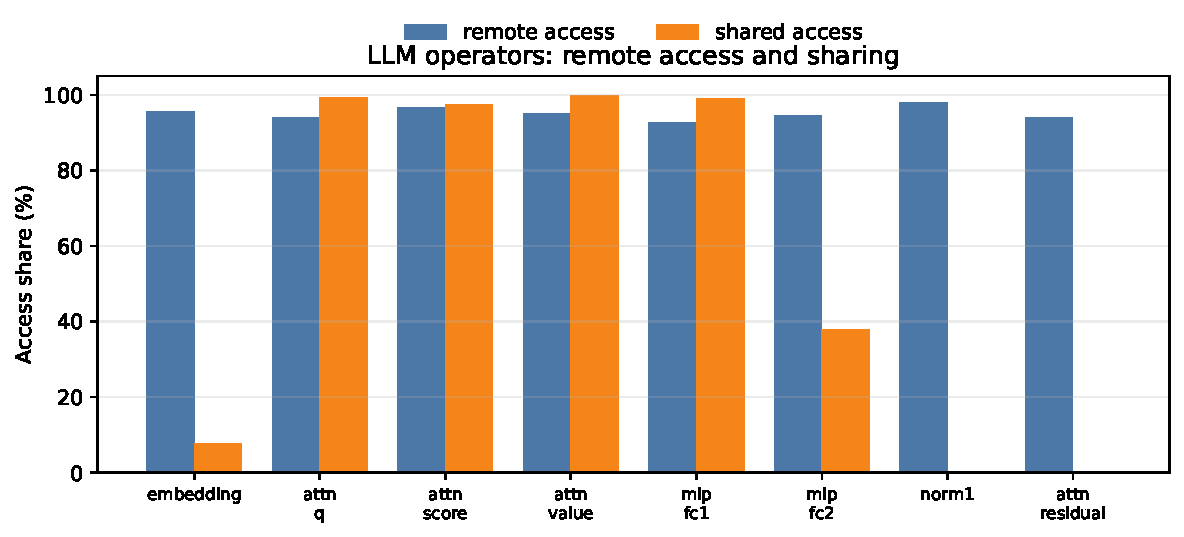
\includegraphics[width=\columnwidth]{figures/llm_remote_shared_bars.pdf}
  \caption{LLM operators often have both high remote-access ratio and high
  shared-access ratio, especially attention projections and MLP fully-connected
  operators.}
  \label{fig:llm-remote-shared}
\end{figure}

The LLM operators show high remote ratios and, for matrix-heavy operators, high
shared-access ratios.  Attention Q/K/V/out and MLP FC1/FC2 are the most
important operators to inspect next because they combine long runtime with high
remote traffic.  However, the current LLM all-local comparison produced
1.0$\times$ speedup for the comparable completed operators.  This means the
current evidence is not sufficient to claim that LLM remote data access is on
the critical path.

The next step for ML workloads is therefore not just more remote-ratio plots.
We need stall attribution and tensor semantics: whether a remote page is a
weight, activation input, activation output, temporary, embedding, or KV/cache
page.  Without tensor labels, page-level sharing can mix weight broadcast,
output placement, temporary buffers, and true shared read-mostly reuse.

\subsection{All LLM Operator Results}

Table~\ref{tab:llm-all} shows all 16 decomposed GPT-7B operators from the
sampled-validation run used for the current LLM analysis.  The matrix-heavy
operators have high remote access and often high shared-access ratios, but this
alone is not a bottleneck proof.

\begin{table*}[t]
  \centering
  \caption{All decomposed GPT-7B operators in the current LLM analysis.  Time is
  driver total time in microseconds.}
  \label{tab:llm-all}
  \resizebox{\textwidth}{!}{\begin{tabular}{lrrrrrrrr}
\toprule
Operator & Time & GPUs & CPI & L1 miss & L2 miss & Remote & Shared acc. & Shared pg. \\
\midrule
embedding & 9.5 & 43 & 14.0 & 100.0 & 99.8 & 95.5 & 7.7 & 0.1 \\
layer00\_norm1 & 38.5 & 4 & 10.9 & 50.0 & 99.3 & 98.0 & 0.0 & 0.0 \\
layer00\_attn\_q & 10941.0 & 47 & 604.6 & 75.6 & 21.8 & 94.0 & 99.5 & 88.2 \\
layer00\_attn\_k & 10941.0 & 47 & 604.6 & 75.6 & 21.8 & 94.0 & 99.5 & 88.2 \\
layer00\_attn\_v & 10941.0 & 47 & 604.6 & 75.6 & 21.8 & 94.0 & 99.5 & 88.2 \\
layer00\_attn\_score & 1919.5 & 16 & 32.7 & 98.0 & 1.8 & 96.7 & 97.4 & 92.1 \\
layer00\_causal\_mask & 4.0 & 2 & 9.6 & 0.0 & 100.0 & 27.5 & 0.0 & 0.0 \\
layer00\_attn\_softmax & 7.9 & 4 & 5.4 & 33.3 & 99.4 & 75.0 & 0.0 & 0.0 \\
layer00\_attn\_value & 164.0 & 47 & 5.2 & 26.7 & 33.3 & 95.1 & 99.8 & 90.7 \\
layer00\_attn\_out & 10941.0 & 47 & 604.6 & 75.6 & 21.8 & 94.0 & 99.5 & 88.2 \\
layer00\_attn\_residual & 8.6 & 43 & 37.2 & 100.0 & 100.0 & 94.1 & 0.0 & 0.0 \\
layer00\_norm2 & 38.5 & 4 & 10.9 & 50.0 & 99.3 & 98.0 & 0.0 & 0.0 \\
layer00\_mlp\_fc1 & 25223.0 & 48 & 1174.5 & 71.7 & 28.5 & 92.7 & 99.0 & 81.1 \\
layer00\_mlp\_gelu & 11.1 & 46 & 13.3 & 100.0 & 99.8 & 84.7 & 0.0 & 0.0 \\
layer00\_mlp\_fc2 & 6842.2 & 47 & 307.6 & 30.3 & 17.9 & 94.6 & 38.0 & 45.0 \\
layer00\_mlp\_residual & 8.6 & 43 & 37.2 & 100.0 & 100.0 & 94.1 & 0.0 & 0.0 \\
\bottomrule
\end{tabular}
}
\end{table*}

\subsection{LLM Bottleneck Oracle}

Table~\ref{tab:llm-bottleneck} reports the completed comparable LLM
all-local-oracle comparison.  The speedups are all 1.0$\times$ in this run.
This does not mean remote data can be ignored.  It means the current oracle does
not expose a performance sensitivity for these operators.  The next LLM run
therefore needs direct stall attribution and page-to-tensor semantic labels.

\begin{table*}[t]
  \centering
  \caption{LLM all-local data oracle comparison.  The current comparable run did
  not show speedup, despite high remote and shared-access ratios.}
  \label{tab:llm-bottleneck}
  \resizebox{\textwidth}{!}{\begin{tabular}{lrrrrr}
\toprule
Operator & Speedup & Remote & Shared acc. & Shared pg. & Accesses \\
\midrule
embedding & 1.00 & 95.5 & 7.7 & 0.1 & 106496 \\
layer00\_norm1 & 1.00 & 98.0 & 0.0 & 0.0 & 98304 \\
layer00\_attn\_q & 1.00 & 94.0 & 99.5 & 88.2 & 1000000 \\
layer00\_attn\_k & 1.00 & 94.0 & 99.5 & 88.2 & 1000000 \\
layer00\_attn\_v & 1.00 & 94.0 & 99.5 & 88.2 & 1000000 \\
layer00\_attn\_score & 1.00 & 96.7 & 97.4 & 92.1 & 1000000 \\
layer00\_causal\_mask & 1.00 & 27.5 & 0.0 & 0.0 & 568 \\
layer00\_attn\_softmax & 1.00 & 75.0 & 0.0 & 0.0 & 4096 \\
layer00\_attn\_value & 1.00 & 95.1 & 99.8 & 90.7 & 1000000 \\
layer00\_attn\_out & 1.00 & 94.0 & 99.5 & 88.2 & 1000000 \\
layer00\_attn\_residual & 1.00 & 94.1 & 0.0 & 0.0 & 98304 \\
layer00\_norm2 & 1.00 & 98.0 & 0.0 & 0.0 & 98304 \\
layer00\_mlp\_fc1 & 1.00 & 92.7 & 99.0 & 81.1 & 1000000 \\
layer00\_mlp\_gelu & 1.00 & 84.7 & 0.0 & 0.0 & 176128 \\
layer00\_mlp\_fc2 & 1.00 & 94.6 & 38.0 & 45.0 & 1000000 \\
layer00\_mlp\_residual & 1.00 & 94.1 & 0.0 & 0.0 & 98304 \\
\bottomrule
\end{tabular}
}
\end{table*}

\subsection{Small LLM Home-L2 Evidence}

A small GPT-7B embedding smoke test produced one concrete shared-read page with
32 requester GPUs, 2048 total read accesses, 1984 remote accesses, and 99.9\%
of remote reads served by remote L2/MSHR rather than remote DRAM.  This is a
good example of the target behavior for selective home-L2 caching.  However, it
is still a smoke-test result.  The full LLM run should be repeated with the new
page-source trace before this becomes a central result.

\section{Research Direction}

\subsection{Remote-Access Taxonomy}

The central direction is to first classify remote traffic and then apply the
right mechanism:

\begin{itemize}
  \item \textbf{Remote-private placement mismatch}: use compute-data
  co-placement or better initial page placement.
  \item \textbf{Remote write/output mismatch}: use output ownership or
  producer-consumer placement.
  \item \textbf{Shared read-mostly reuse}: use selective home-L2 caching.
  \item \textbf{Topology-local neighbor reuse}: use neighbor-exposed L2 service.
\end{itemize}

\subsection{Selective Home-L2 Caching}

Home-L2 caching should target pages with high read ratio, multiple sharers,
enough remote reads, and low write activity.  This avoids treating placement
mismatch as data sharing.

\subsection{Neighbor-Exposed L2}

The more architecture-oriented idea is to split L2 service into a local path and
a neighbor-facing path.  The local path serves the owning GPU with high
priority, while the neighbor path exposes selected lines/pages to north, south,
east, and west neighbors through separate queues or bandwidth.  This is not page
migration and not global coherence.  It is a bounded, topology-aware
memory-hierarchy extension.  SpMV, FWT, FIR, and SimpleConv provide the strongest
early evidence for this path.

\subsection{Cross-GPU Translation Prefetching}

Cross-GPU translation prefetching was considered as an auxiliary mechanism.  It
can pre-populate translation and owner metadata for remote pages, reducing TLB
and IOMMU lookup overhead.  It does not by itself solve remote data movement or
remote DRAM pressure.  The current conclusion is that translation prefetching is
best treated as support for home-L2 or neighbor-L2 policies, not as the main
contribution.

\subsection{Why MatMul Is a Negative Control}

MatMul is useful precisely because it looks promising under a simple remote
ratio metric but does not benefit under the all-local oracle.  It has 89.0\%
remote accesses and 97.6\% shared-read-mostly remote traffic, but remote reads
are almost entirely served by L2/MSHR, the neighbor-read ratio is only 5.2\%,
and the oracle speedup is about 1.0$\times$.  This argues that future designs
must be selective and performance-aware.

\section{Current Claims}

Based on this week's evidence, the strongest claims are:

\begin{enumerate}
  \item Remote traffic on wafer-scale GPUs is heterogeneous; remote-access ratio
  alone is not a reliable optimization signal.
  \item SpMV currently provides the clearest evidence that remote data movement
  can be a performance bottleneck.
  \item PageRank provides the clearest evidence for shared-read home-L2 style
  reuse.
  \item FWT and FIR provide evidence for topology-local neighbor-facing L2
  service.
  \item MatMul and AES are important negative controls, showing that high remote
  traffic or high sharing can still produce little performance sensitivity.
  \item For LLM operators, high remote and shared-access ratios are visible, but
  the current oracle does not prove remote data is on the critical path.
\end{enumerate}

\section{Next Week Plan}

\begin{enumerate}
  \item Rerun the full LLM decomposed workload with \texttt{--trace-sharing} and
  \texttt{--report-l2-source}, then analyze
  \texttt{l2\_home\_evidence\_summary.csv}.
  \item Add stall attribution: remote memory stall cycles, translation stall
  cycles, NoC/RDMA wait, and DRAM queue wait.
  \item Add tensor-semantic labels for ML pages: weight, input activation,
  output activation, temporary, embedding, and KV/cache.
  \item Implement a neighbor-L2 oracle in which 1-hop remote L2/MSHR service
  receives reduced latency or isolated bandwidth.
  \item Use SpMV, PageRank, FWT, FIR, MatMul, and AES as the core benchmark set:
  SpMV and PageRank as positive cases, FWT/FIR as neighbor cases, and
  MatMul/AES as negative controls.
\end{enumerate}

\section{Commands}

\subsection{Traditional Workload Trace}

\begin{verbatim}
cd /home/daoxuanxu/dataSharing/WSG-baseline-model/akkalat

python3 runall2.py \
  --benchmarks traditional \
  --configs baseline \
  --disable-servers \
  --trace-sharing \
  --trace-sharing-sample 1 \
  --trace-sharing-max-records 0 \
  --report-l2-source \
  --l2-source-tile-width 7 \
  --max-workers 10
\end{verbatim}

\subsection{LLM Decomposed Trace}

\begin{verbatim}
cd /home/daoxuanxu/dataSharing/WSG-baseline-model/akkalat

python3 runllm_decomposed.py \
  --model gpt \
  --profile gpt-7b \
  --layers 1 \
  --seq-len 128 \
  --split-k 8 \
  --configs llm_mixed \
  --sampled-warmup 128 \
  --sampled-granularity 512 \
  --disable-servers \
  --trace-sharing \
  --trace-sharing-sample 1 \
  --trace-sharing-max-records 1000000 \
  --report-l2-source \
  --l2-source-tile-width 7 \
  --max-workers 10 \
  --summarize
\end{verbatim}

\balance
\end{document}
